\chapter{A Gallery of Some 3D Representations of Feral
  Knots}\label{chap:feral-gallery}
\def\figdir{figures/feral-gallery}
\def\otherfigdir{figures/unknotting-moves-and-combinatorial-representations}
The following theorem is proven in \cite{Crowell1963} (Appendix I,
pg.\ 147).
\begin{theorem}\label{thm:c1-suffices}
  Let $K$ be a knot in $\RR^3$ which is rectifiable and which is given
  as the image of a periodic vector-valued function $p(s) = (x(s),
  y(s), z(s))$ of arc length $s$ whose derivative $p'(s) = (x'(s),
  y'(s), z'(s))$ exists and is continuous for all $s$. Then $K$ is
  tame.
\end{theorem}
From what we can tell, the rectifiability condition is actually
superfluous, as it follows directly from the $C^1$ hypothesis. $C^1$
implies bounded variation, which in turn implies rectifiability. We
imagine \cite{Crowell1963} were simply trying to keep the prerequisite
knowledge to a minimum. In any case, we restate the result as follows.
\begin{theorem}
  Let $K : S^1\into \RR^3$. Then if $K$ is $C^1$, $K$ is tame.
\end{theorem}
We'll cite this freely in the below.


\section{Countable Twists}
\begin{example}[Countable Twists]~
  \begin{itemize}
    \item Description: A countable \# of twists
    \item Example countable polygonal representation
      \begin{figure}[H]
        \centering
        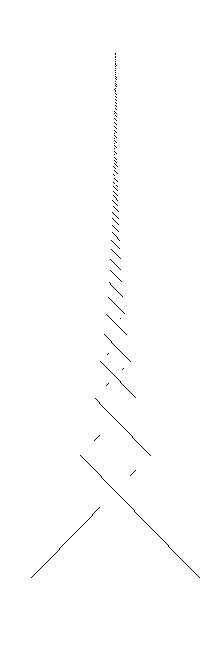
\includegraphics[angle=-90]{\otherfigdir/countable-r1-v2.pdf}
        \caption{Countable Polygonal Representation}
      \end{figure}
    \item Proof of tameness, method 1: Use Reidemeister I moves and
      \cref{thm:uniformly-convergent-ambient-isotopy}
    \item Proof of tameness, method 2: Explicit, $C^1$ 3D parameterization
      as an arc: $f : [-\pi,\pi] \into \RR^3$, parameters $r, \omega$.
      \[
      f(\theta) =
      \begin{cases}
        \begin{bmatrix}
          r \theta^3 \cos\pn{\frac{\omega}{\theta}} \\
          r \theta^3 \sin\pn{\frac{\omega}{\theta}} \\
          \theta^2
        \end{bmatrix} & \theta \geq 0 \\
        -f(-\theta) & \theta < 0
      \end{cases}
      \]
      $C^1$: all of $(-\pi, \pi)$. Can be extended past $\pm \pi$
      easily.
      \begin{figure}[H]
        \centering
        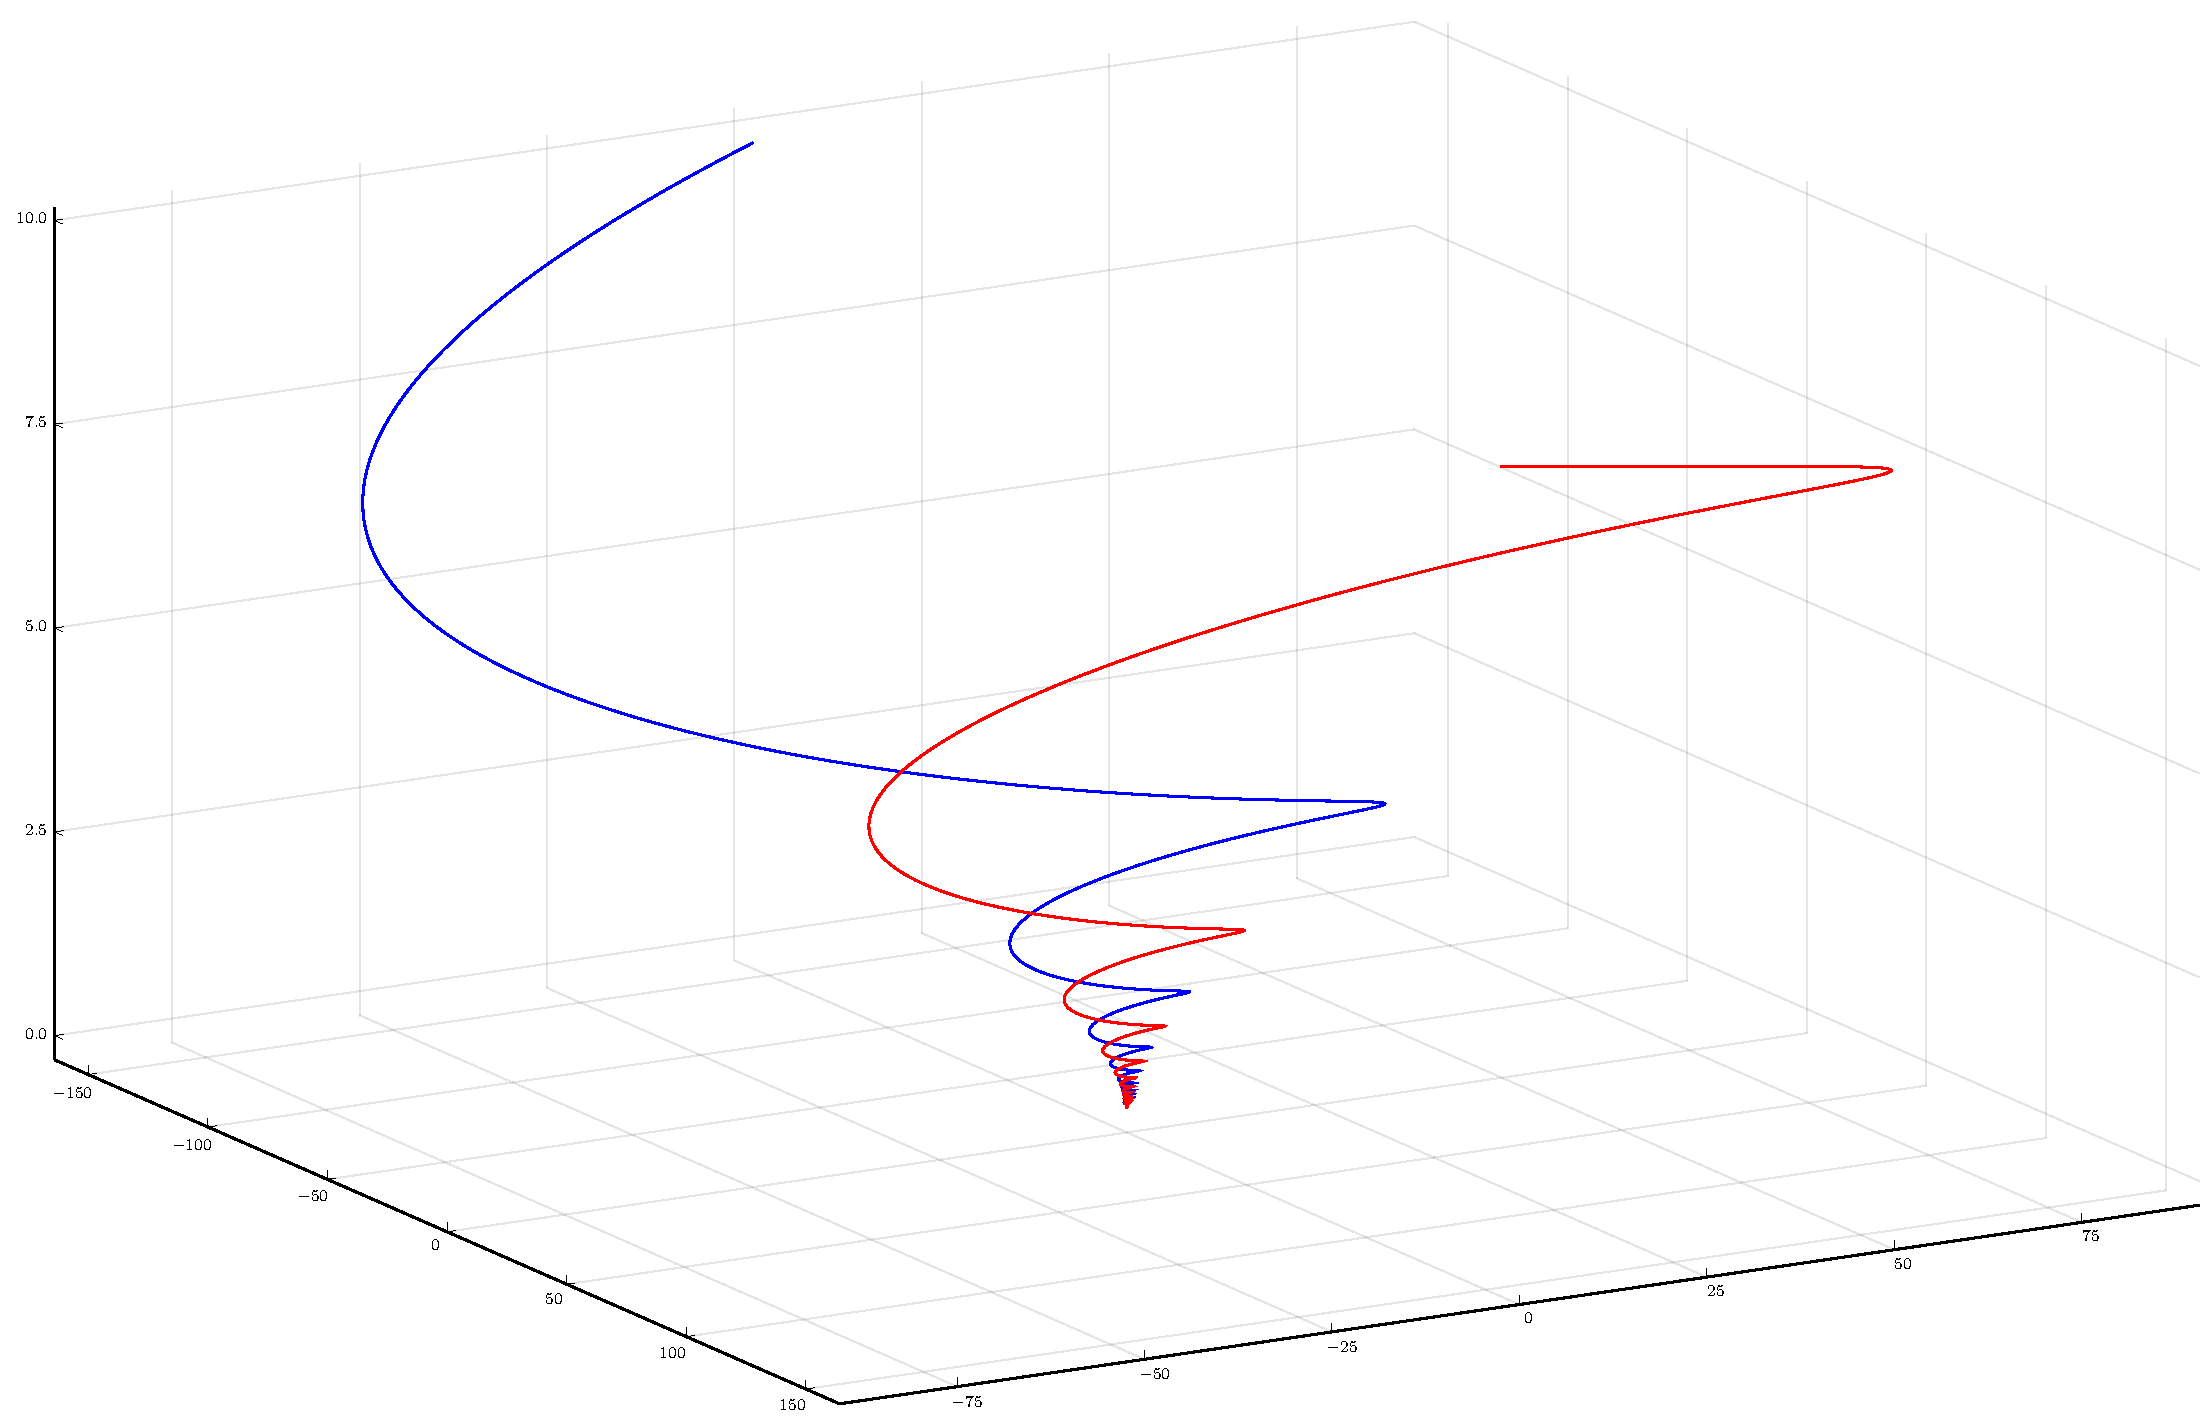
\includegraphics[scale=.25]{\figdir/countable-3d-twists-side.pdf}
        \caption{Perspective view}
        \label{fig:twists-perspective}
      \end{figure}
      \begin{figure}[H]
        \centering
        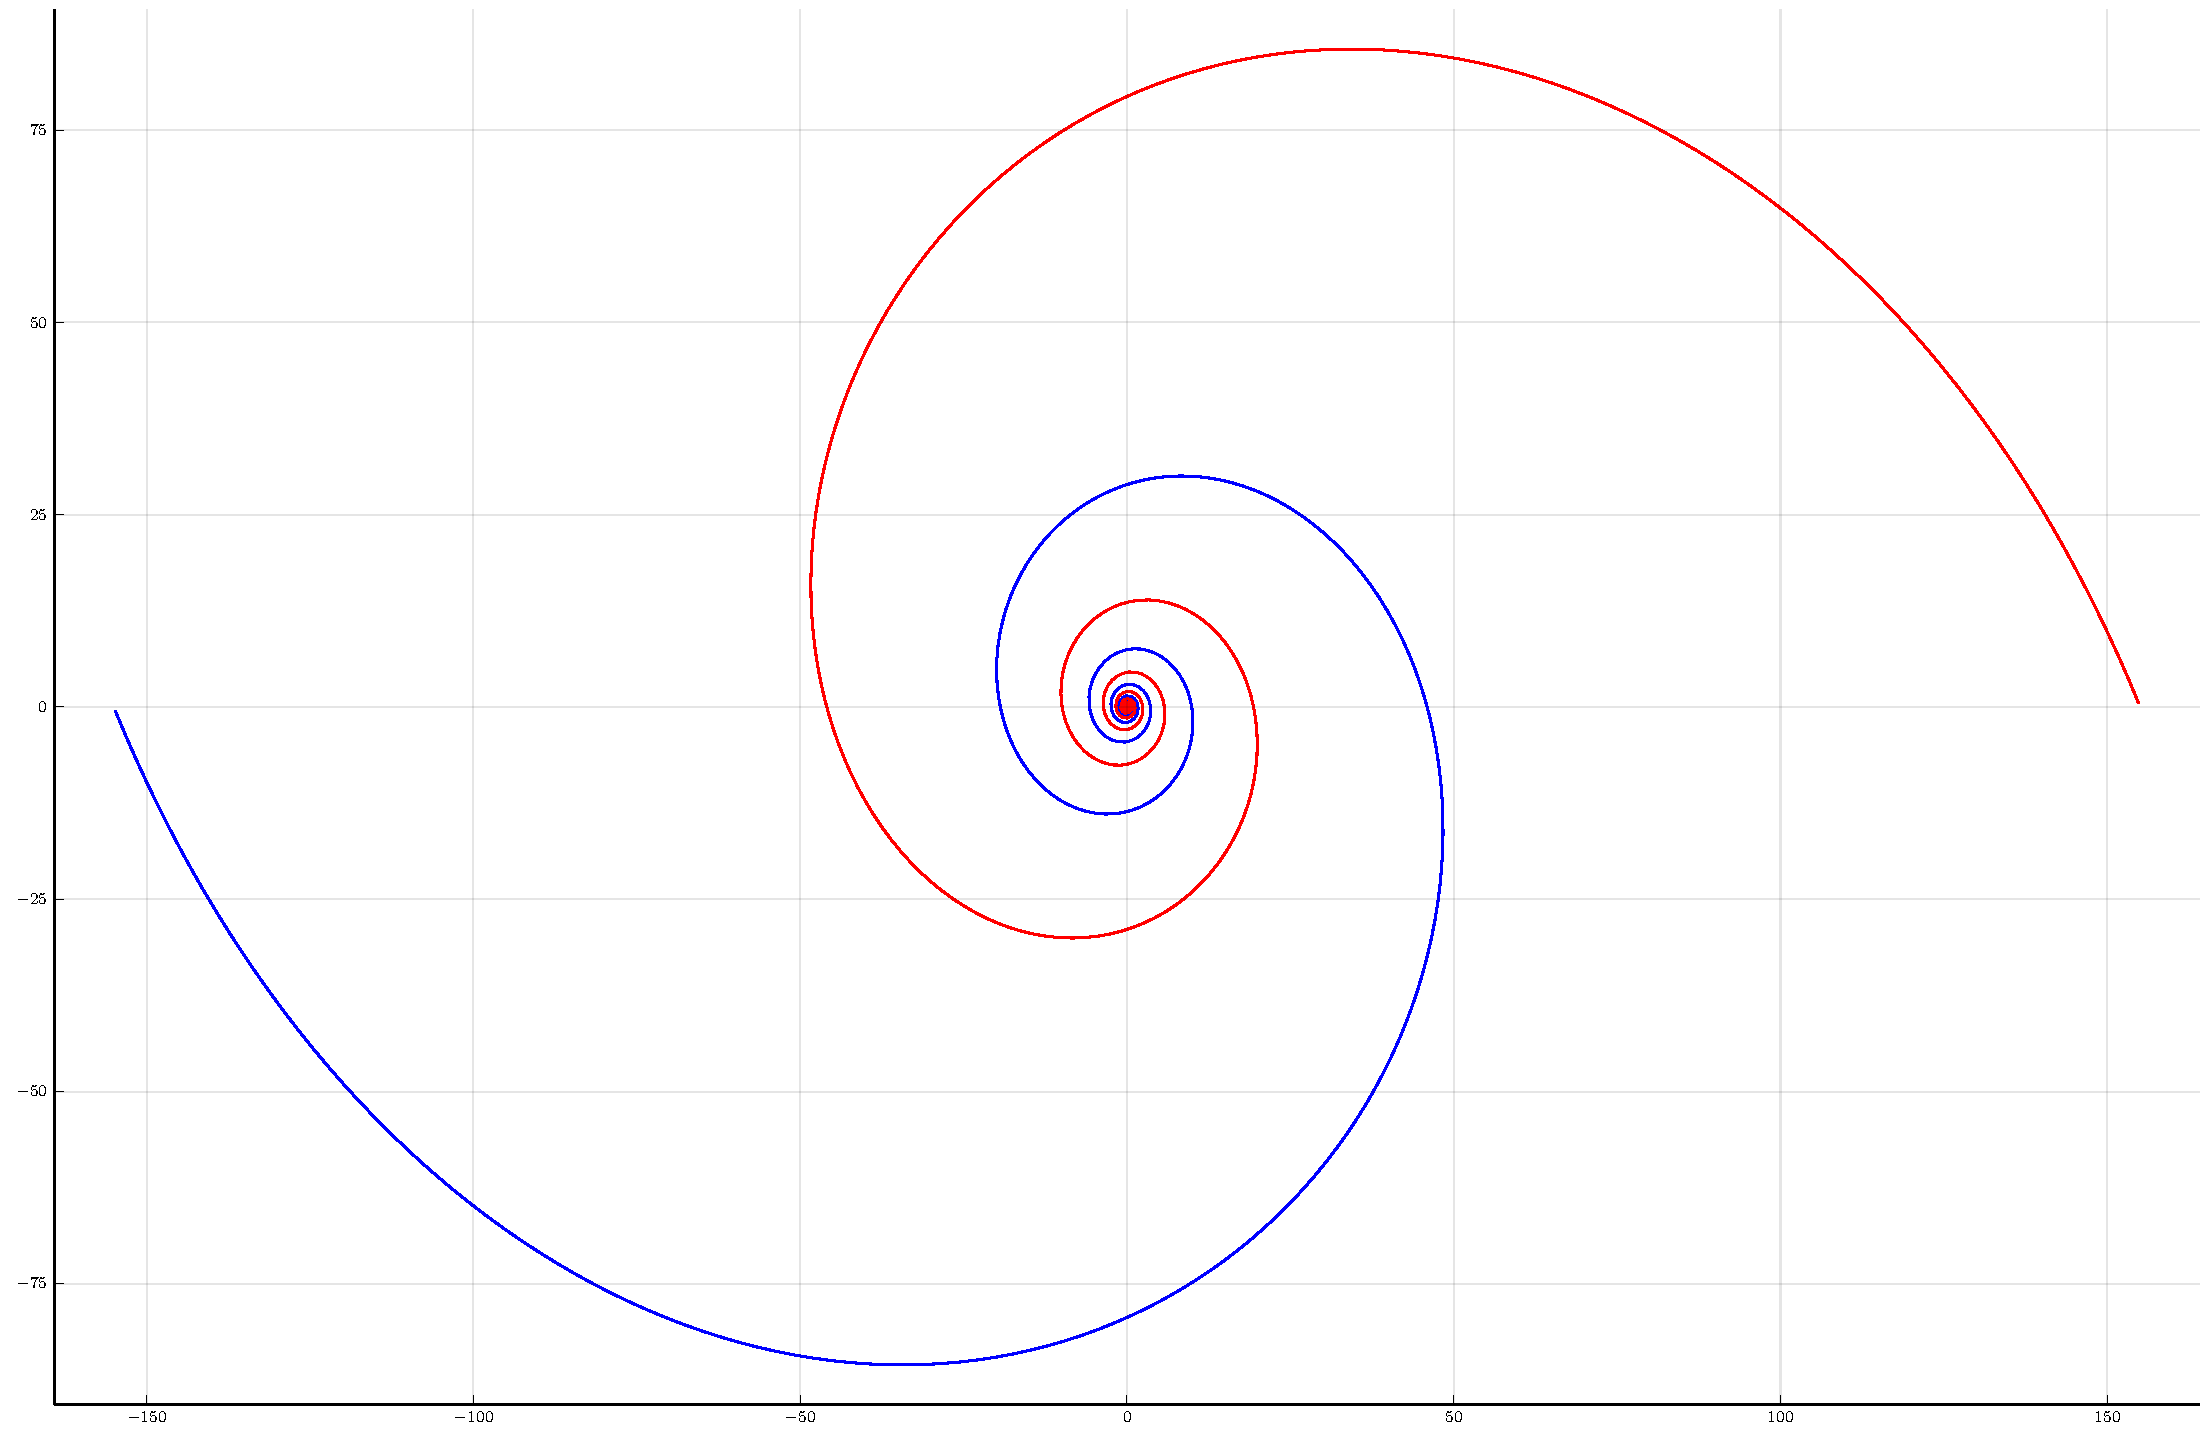
\includegraphics[scale=.25]{\figdir/countable-3d-twists-top.pdf}
        \caption{Top view}
        \label{fig:twists-top}
      \end{figure}
    \item Proof of tameness, method 3: Employ the top-down view and
      apply \cref{prop:replacing-by-same-endpoints}.
  \end{itemize}
\end{example}

\section{Countable Reidemeister II}
\begin{example}[Countable Reidemeister II]~
  \begin{itemize}
    \item Description: A countable \# of Reidemeister II's
    \item Example countable polygonal representation
      \begin{figure}[H]
        \centering
        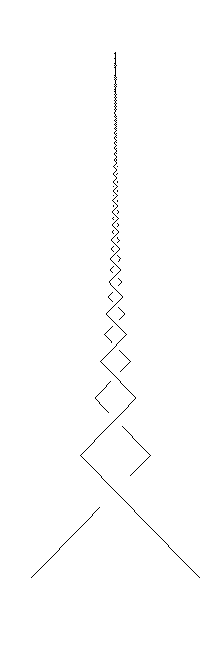
\includegraphics[angle=-90]{\otherfigdir/countable-r2-v2.pdf}
        \caption{Countable Polygonal Representation}
      \end{figure}
    \item Proof of tameness, method 1: Use Reidemeister II moves and
      \cref{thm:uniformly-convergent-ambient-isotopy}, or
      alternatively, using
      \cref{thm:countable-gluing-ambient-isotopies} in two steps.
    \item Proof of tameness, method 2: Explicit, $C^1$ 3D parameterization
      as an arc: $f : [-\pi,\pi] \into \RR^3$, parameters $r, \omega$.
      \[
      f(\theta) =
      \begin{cases}
        \begin{bmatrix}
          r \theta^3 \cos\pn{\frac{\omega}{\theta}} \\
          \theta^2
          \theta^2
        \end{bmatrix} & \theta \geq 0 \\
        \begin{bmatrix}
          -r \theta^3 \cos\pn{\frac{\omega}{\theta}} \\
          -\theta^2
          \theta^2
        \end{bmatrix} & \theta < 0
      \end{cases}
      \]
      $C^1$: everywhere on $(-\pi, \pi)$. Can be extended past $\pm
      \pi$ easily.
      \begin{figure}[H]
        \centering
        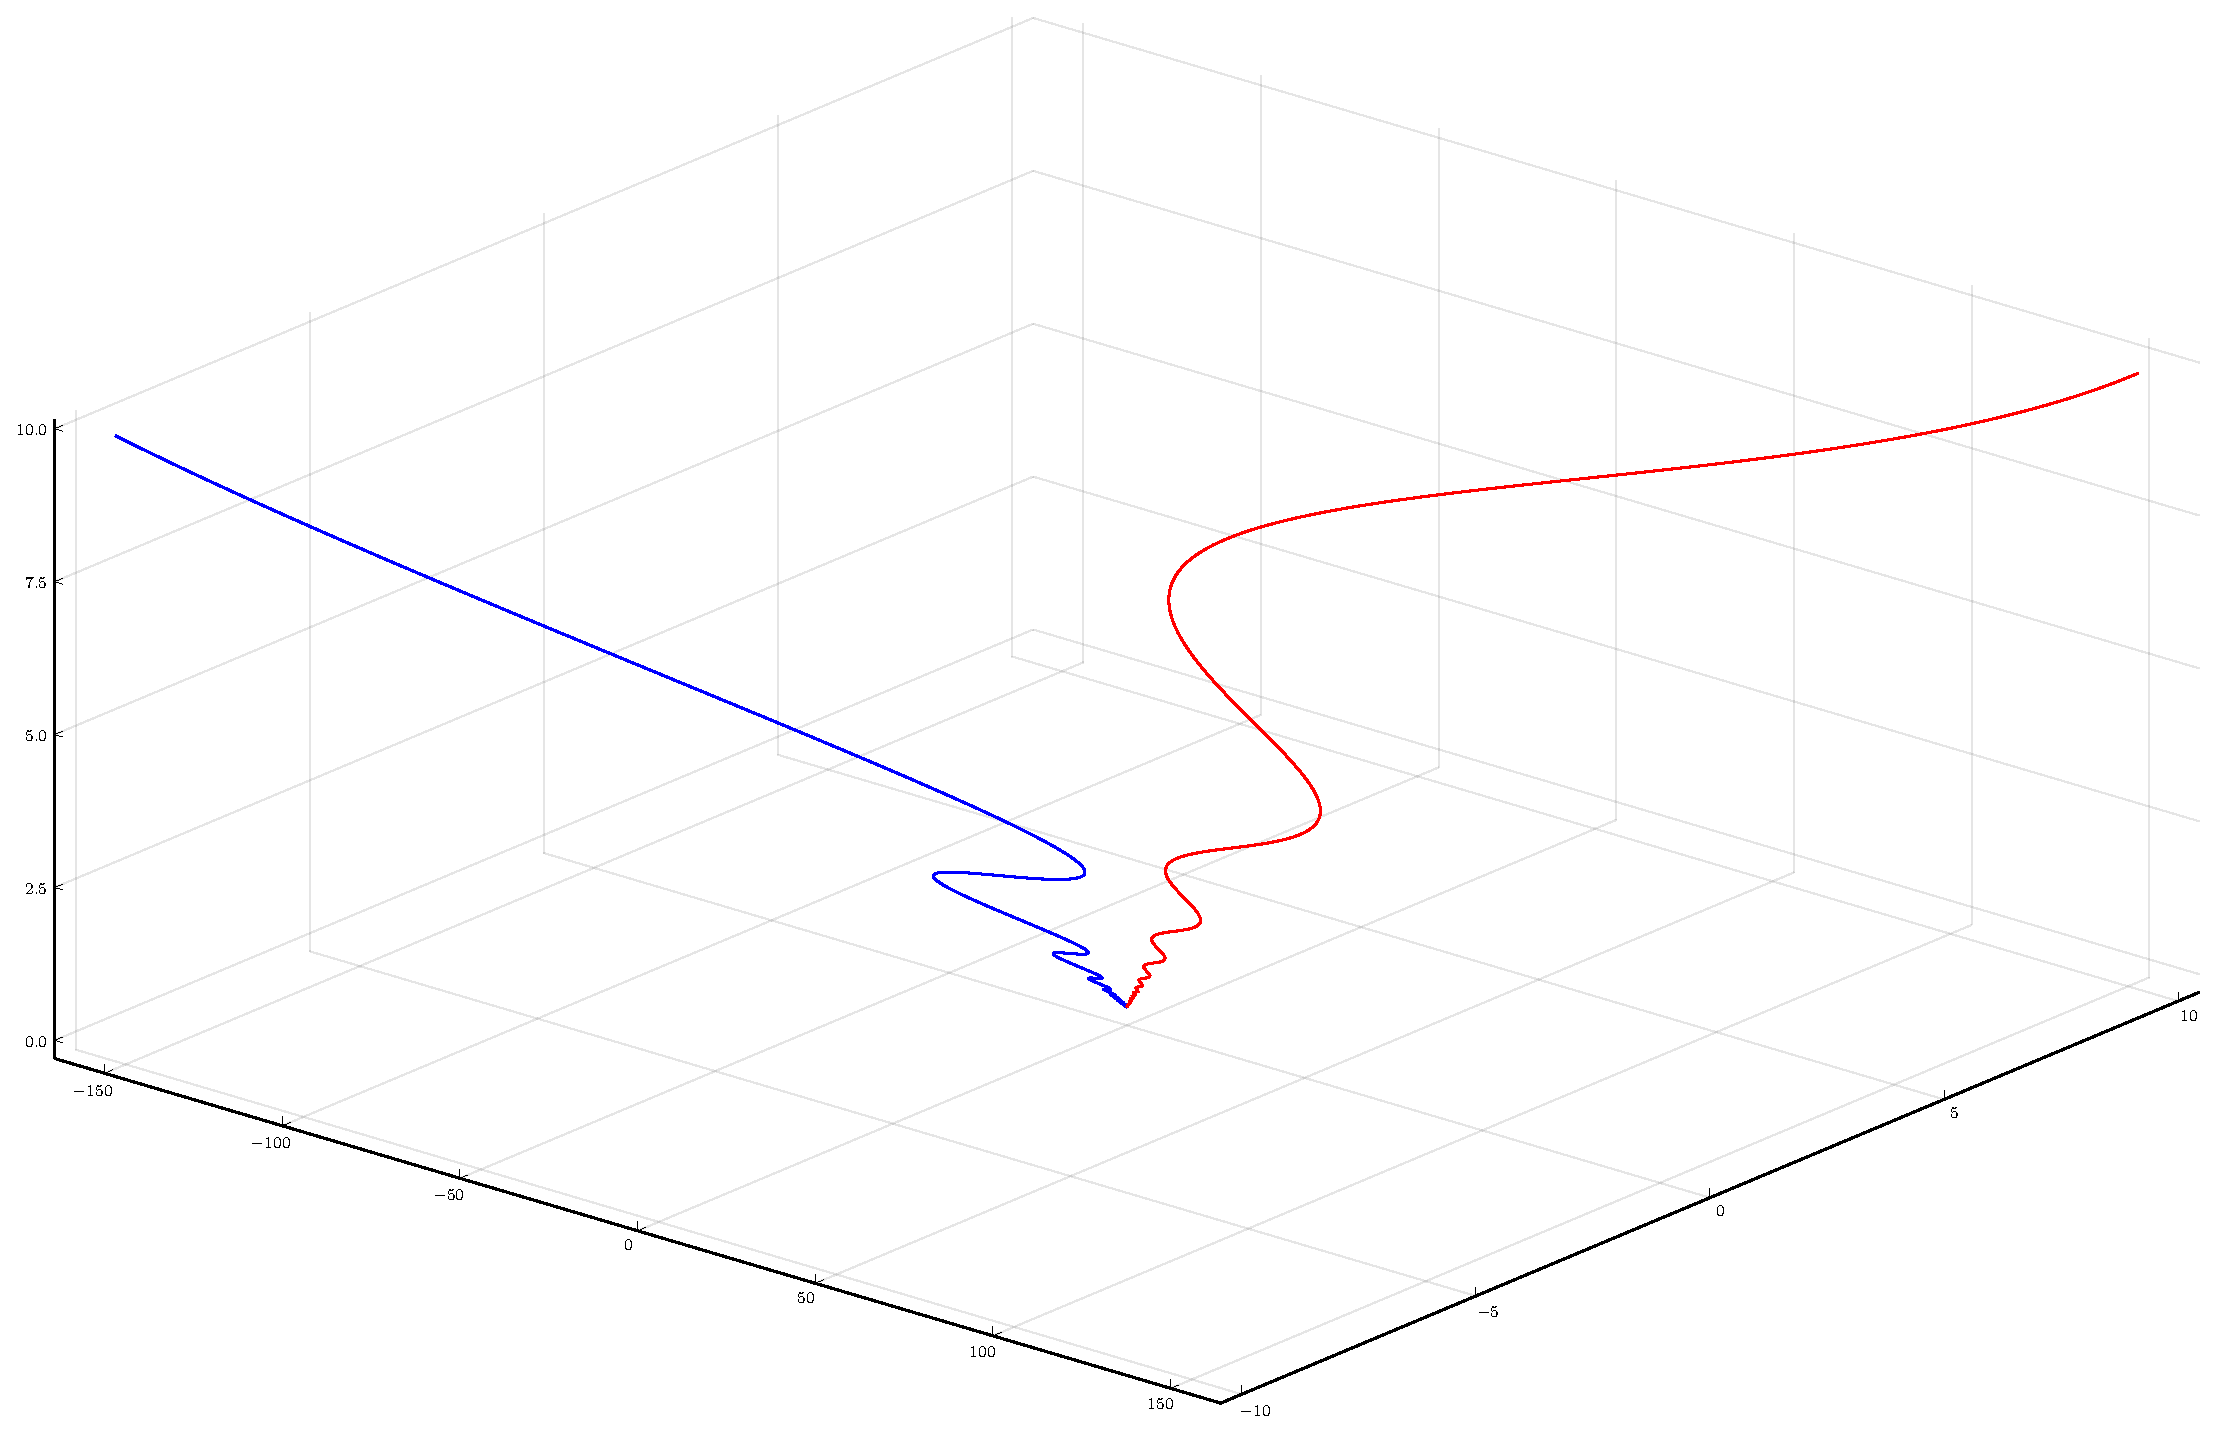
\includegraphics[scale=.25]{\figdir/countable-3d-r2-perspective.pdf}
        \caption{Perspective view}
        \label{fig:countable-r2-perspective}
      \end{figure}
      \begin{figure}[H]
        \centering
        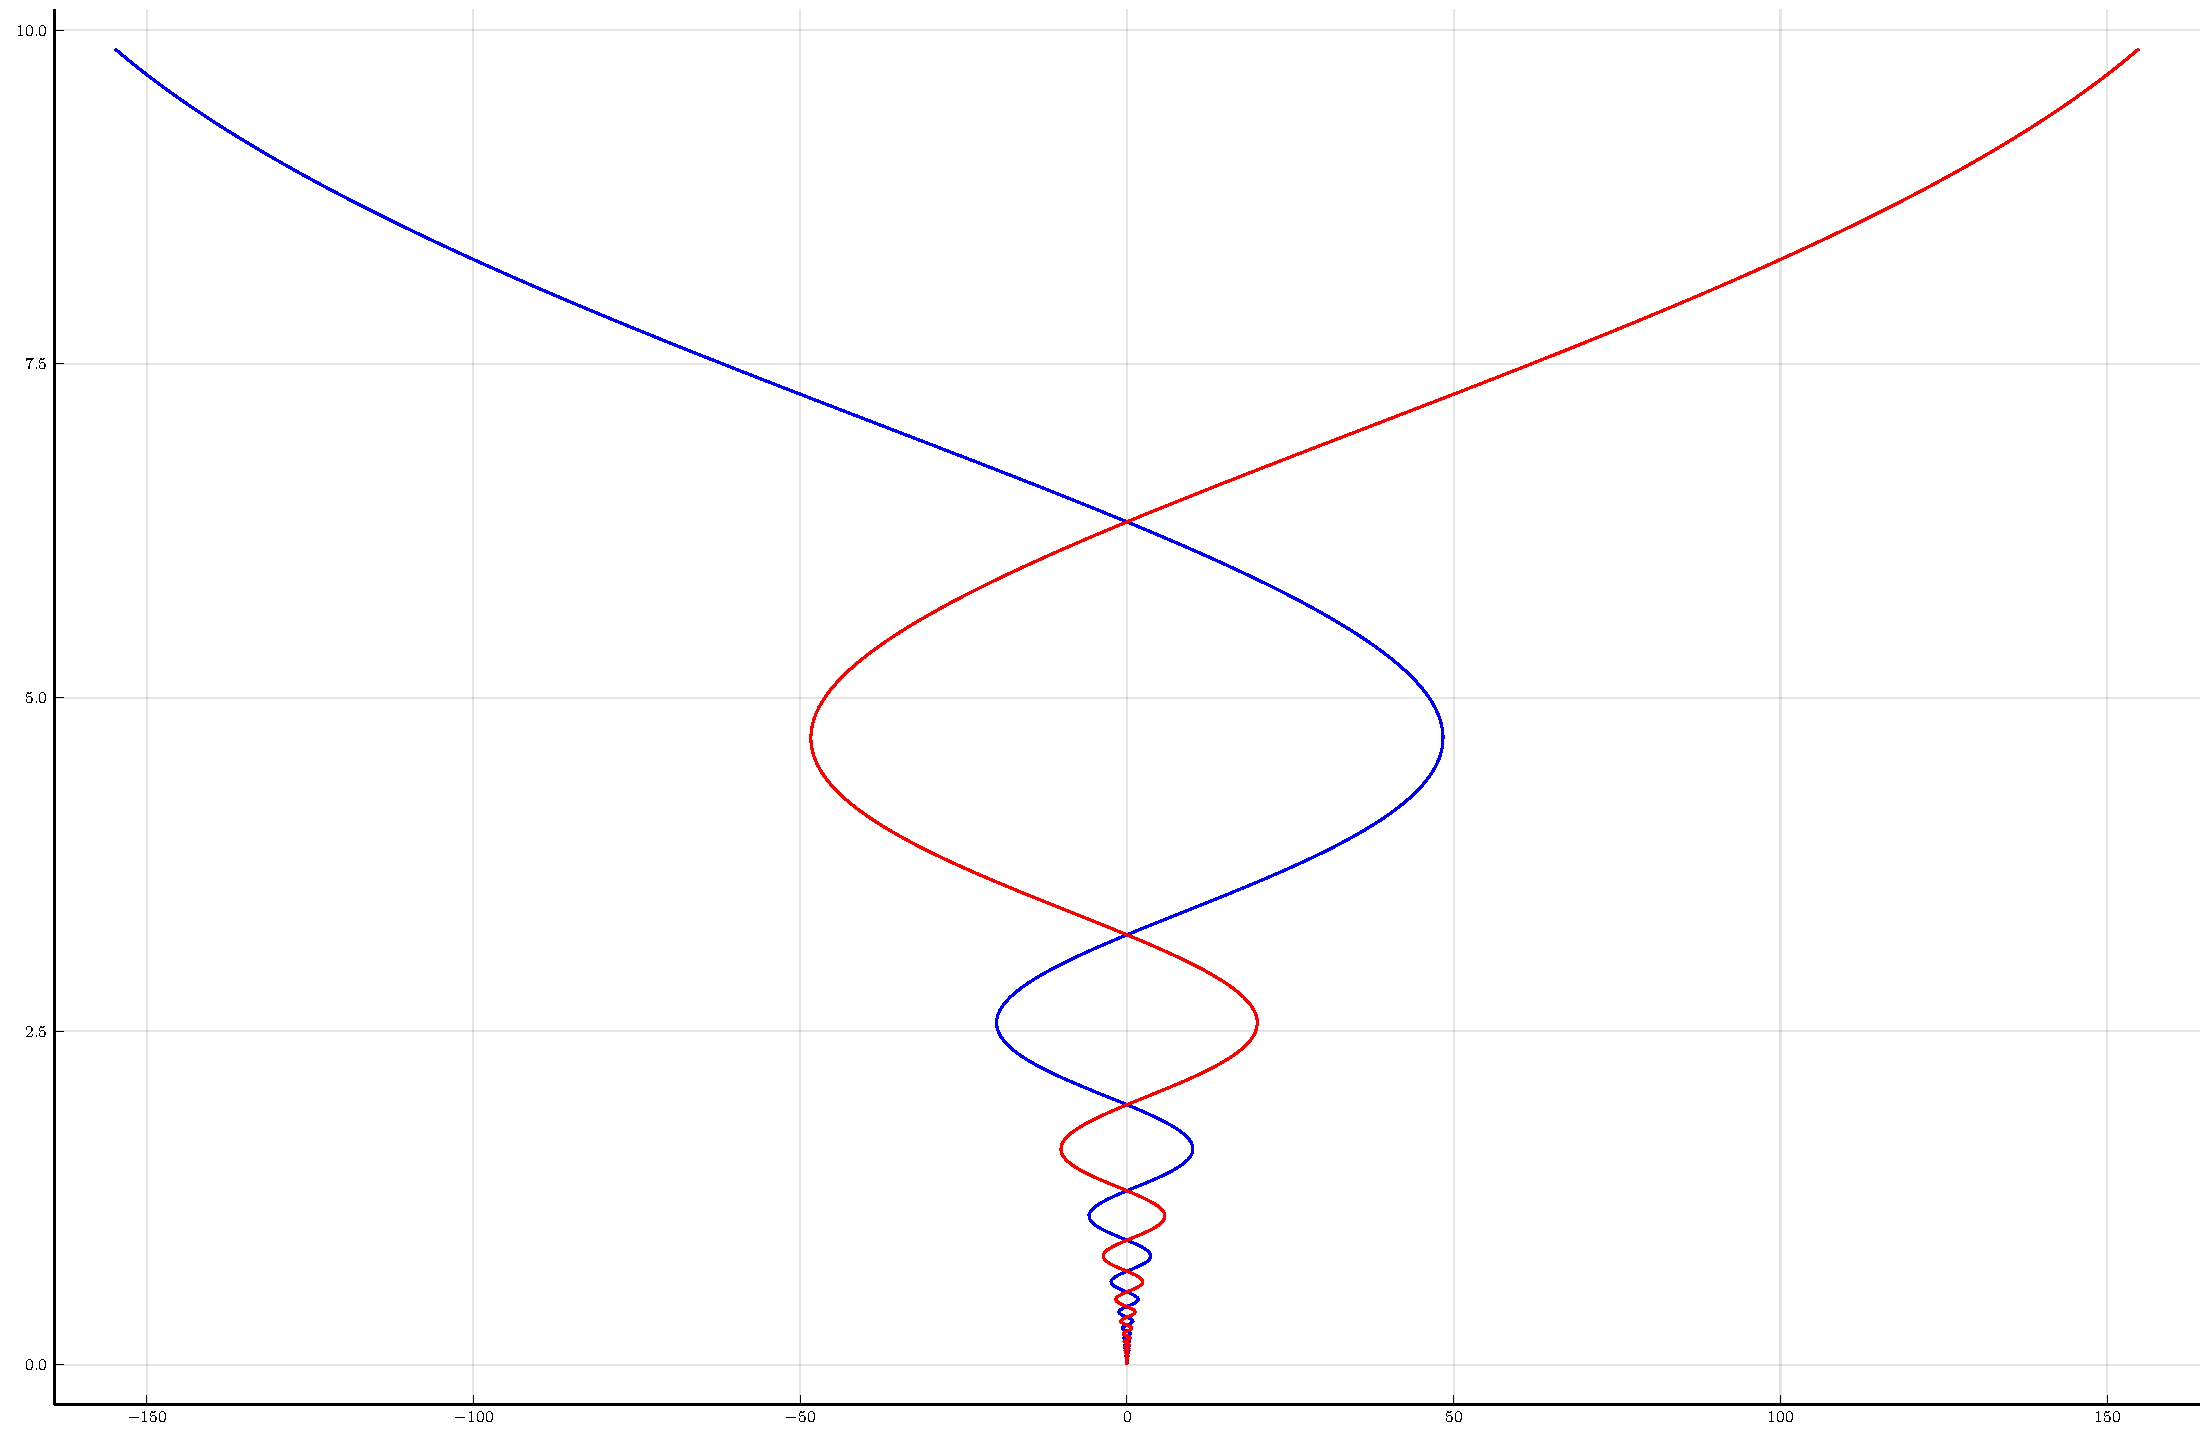
\includegraphics[scale=.25]{\figdir/countable-3d-r2-side.pdf}
        \caption{Side view}
        \label{fig:countable-r2-side}
      \end{figure}
      \begin{figure}[H]
        \centering
        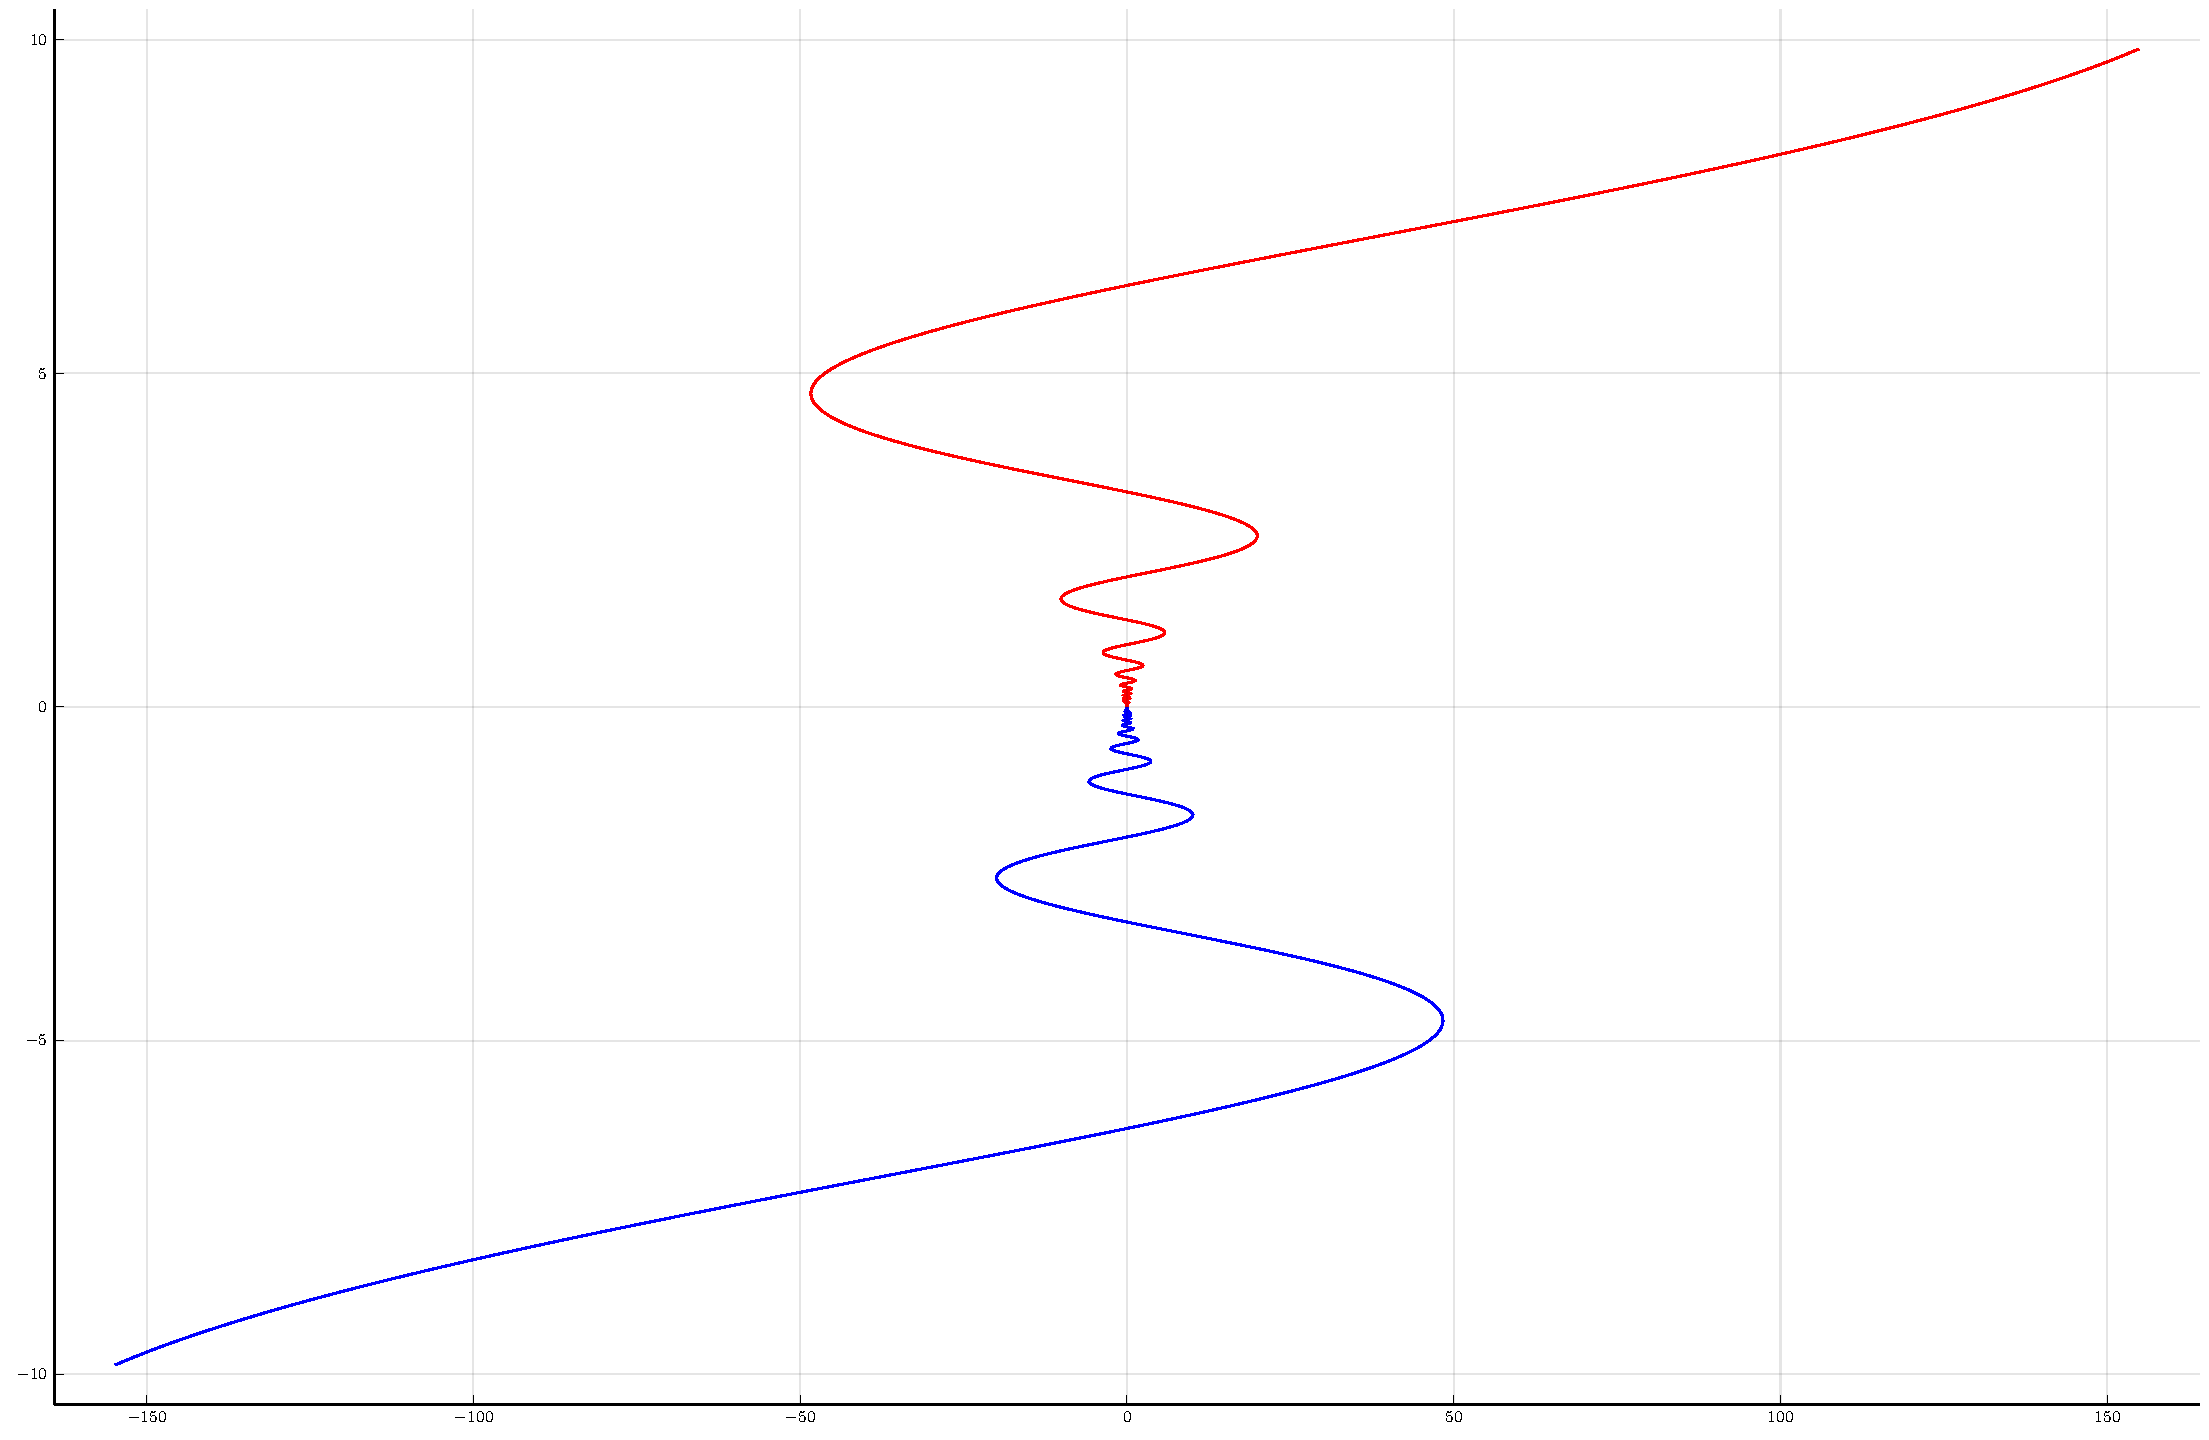
\includegraphics[scale=.25]{\figdir/countable-3d-r2-top.pdf}
        \caption{Top view}
      \end{figure}
    \item Proof of tameness, method 3: Employ the top-down view and
      apply \cref{prop:replacing-by-same-endpoints}.
  \end{itemize}
\end{example}







%%% Local Variables:
%%% TeX-master: "../../kobayashi-thesis"
%%% End:
